\documentclass[11pt]{article}

\usepackage[english]{babel}
\usepackage[utf8]{inputenc}
\usepackage{amsmath, amsthm, amssymb}
\usepackage{graphicx}


\title{User documentation}

\author{Martin Münch, Marcel Ouška}

\date{20. 5. 2014}

\begin{document}

\maketitle

\section{Device description}
As you can see on picture, device is composed only from keyboard and LCD display. It's main purpose is to provide security system for door.

\begin{figure}[ht!]
\centering
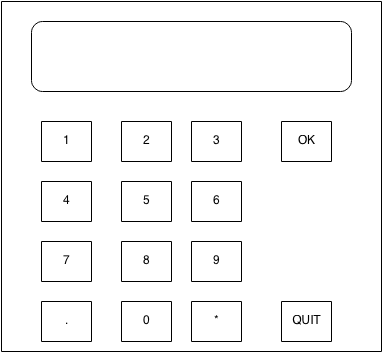
\includegraphics[width=50mm]{apo}
\caption{Device}
\label{overflow}
\end{figure}

When you access door with this device, you will see on display ``INSERT ID''. After you write your ID, push key OK. Next you are asked to ``INSERT PIN'', after inserting pin, push key OK once again. Ater that, communication with server will happen and either you see ``ACCESS GRANTED'' and you can carry on through the door or you will see error message and hear 3 long beeps. Here is table with error messages: 

Při přistoupení k dveřím je na LCD zobrazeno INSERT ID:. Uživatel zadá ID a potvrdí stiskem klávesy OK. Pak je textem INSERT PIN vyzván k zadání kódu. Poté proběhne komunikace se serverem a při správných údajích vypíše ACCESS GRANTED a jednou krátce pípne. Při špatných údajích vypíše jinou hlášku a 3x dlouze zapíská. Chybové hlášky jsou vidět v tabulce. 

\begin{table}[h]
\begin{tabular}{ll}
Message             & meaning            \\ 
UNKNOWN ID      & You wrote ID which is not found in the authorised personel database     \\ 
UNKNOWN PIN     & You wrote incorrect PIN code       \\
NOT AUTHORIZED  & Your credentials are correct, but you are not authorised to access this door \\
UNKNOWN COMMAND &  Unexoected situation happend, try again
\end{tabular}
\end{table}

In case you want to turn off the device, just hold key QUIT. (Despite you won't be able to go through door')

\end{document}